In this section, I will outline the method chosen to perform simulations for both the top and stop decays, from generator level simulations to the detector simulations. 

%-------------------------------------------------------------------------%
\section{Background and Signal of interest}

As discussed earlier, MadGraph5 is the chosen software to perform particle collider simulations, in which one million events were produced. At the generator level, in order to meet the pre-selection criteria, 

Since the decay process involves both leptonic and hadronic particles, the following were defined in order to make the simulation complete.

\begin{lstlisting}[mathescape = true]
        define leptonic = l+ l- ta+ ta- vl vl$\sim$
        define hadronic = u c d s u$\sim$ c$\sim$ d$\sim$ s$\sim$ b b$\sim$
\end{lstlisting}


\begin{equation}
 pp \rightarrow t \Bar{t} \rightarrow b\Bar{b}l^{+}jj\cancel{\it{E}}_{T}
 \label{eq:background}
\end{equation}


\begin{lstlisting}[mathescape = true]
        generate p p > t t$\sim$ , 
        (t > W+ b , W+ > leptonic leptonic),
        (t$\sim$ > W- b$\sim$, W- > hadronic hadronic)
        
        add process p p > t1 t1$\sim$ , 
        (t > W+ b , W+ > hadronic hadronic)), 
        (t$\sim$ > W- b$\sim$, W- > leptonic leptonic)
\end{lstlisting}


\begin{figure}[htbp]
    \centering
    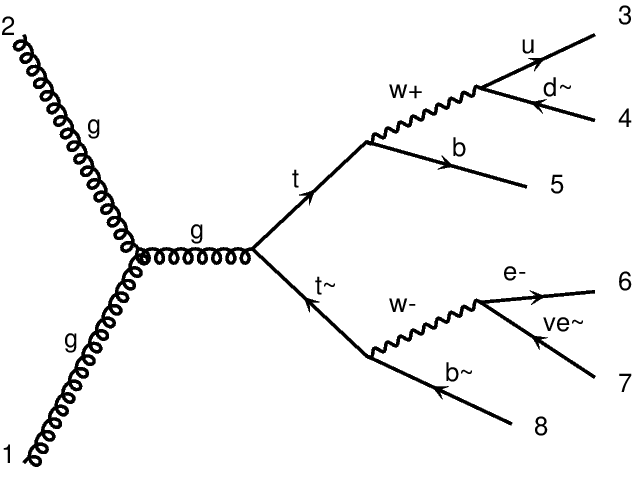
\includegraphics[width=8cm, height= 6.5cm]{top_MG5.png}
    \caption{Feynman diagram of the leading order background process $pp \rightarrow t \Bar{t} \rightarrow b\Bar{b}l^{+}jj\cancel{\it{E}}_{T} $}
    \label{fig:bkrdFeyn}
\end{figure}



\begin{equation}
  pp \rightarrow \Tilde{t}\Tilde{t^*} \rightarrow t \Bar{t} \Tilde{\chi^0_1}\Tilde{\chi^0_1} \rightarrow b\Bar{b}l^{+}jj\cancel{\it{E}}_{T}
  \label{eq:signal}
\end{equation}


\begin{lstlisting}[mathescape = true]
         generate p p > t1 t1$\sim$ ,
        (t1 > t n1, (t > W+ b , W+ > leptonic leptonic)),
        (t1~ > t$\sim$ n1, (t$\sim$ > W- b$\sim$, W- > hadronic hadronic))
        
        add process p p > t1 t1$\sim$ , 
        (t1 > t n1, (t > W+ b , W+ > hadronic hadronic)), 
        (t1$\sim$ > t$\sim$ n1, (t$\sim$ > W- b$\sim$, W- > leptonic leptonic))
\end{lstlisting}



\begin{figure}[htbp]
    \centering
    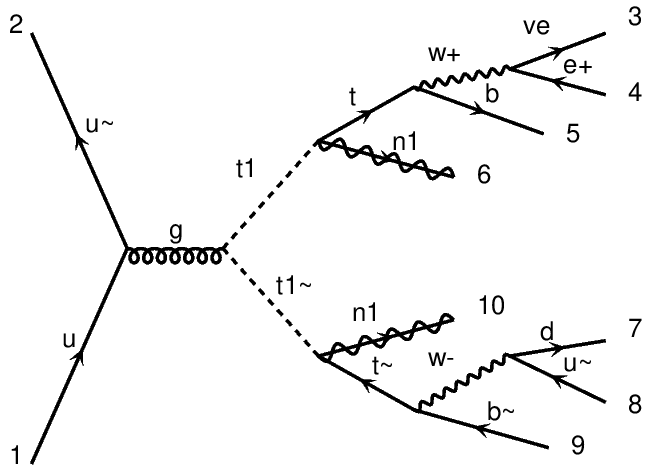
\includegraphics[width=8cm, height= 6.5cm]{stop_MG5.png}
    \caption{Feynman diagram of the leading order signal process $ pp \rightarrow \Tilde{t}\Tilde{t^*} \rightarrow t \Bar{t} \chi^0_1\chi^0_1 \rightarrow b\Bar{b}l^{+}jj\cancel{\it{E}}_{T} $ where the final states are identical to that of the background in Figure \ref{fig:bkrdFeyn}. }
    \label{fig:sigFeyn}
\end{figure}

%as expected from the input equation (\ref{eq:signal}).
%-------------------------------------------------------------------------%
%\subsection{}

%-------------------------------------------------------------------------%
\section{Parton Showers with Pythia and detector simulation with Delphes}


%-------------------------------------------------------------------------%
\section{Kinematic variables in collider experiments}


\begin{figure}[htbp]
    \centering
    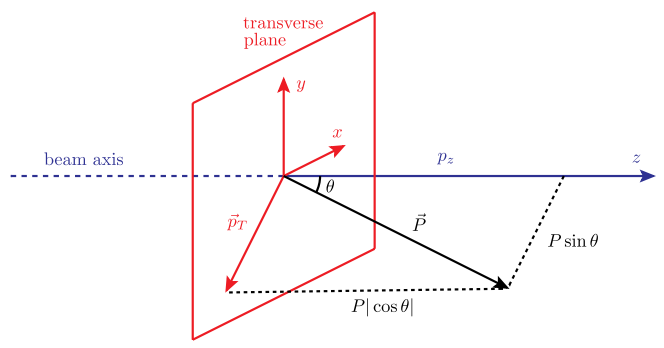
\includegraphics[width=12cm, height= 6cm]{beam.png}
    \caption{The geometry of a collider experiment, with the beam axis considered as the z-direction and the transverse plane as the $(x,y)$-plane \cite{barr2011guide}.}
    \label{fig:beam}
\end{figure}
 given by Equation (\ref{eq:pt})
\begin{equation}
    p_T = \sqrt{p_x^2 + p_y^2}
    \label{eq:pt}
\end{equation}

\begin{figure}[htbp]
    \centering
    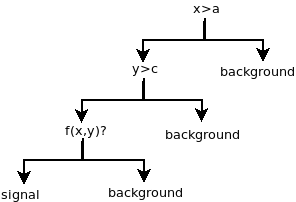
\includegraphics[width=8cm, height= 6cm]{Diagram2.png}
    \caption{Diagram depicting the flow of a cut-based analysis with arbitrary cuts $x$, $y$ and $f(x,y)$, where the final outcome has maximized SNR.}
    \label{fig:cut}
\end{figure}
